\documentclass{beamer}
\usetheme{metropolis}

\usepackage[ngerman]{babel}
\usepackage[autostyle=true,german=quotes]{csquotes}
\usepackage[linewidth=1pt]{mdframed}
\usepackage{hyperref}
\usepackage{makecell}
\usepackage{pifont}
\usepackage{tikz}
\usetikzlibrary{positioning, calc, arrows, fit, decorations.pathreplacing, shapes, shapes.multipart, snakes}
\usepackage{verbatim}
\usepackage{textcomp}
\usepackage{centernot}
\usepackage{tabularx}
\usepackage{ulem}
%\usepackage{pdfpages}

\batchmode

\hypersetup{
	colorlinks,
	urlcolor=blue,
	linkcolor=black % for ToC
}
\newenvironment{qaa}[1]{
	#1

	\begin{mdframed}
		\small
}{
	\end{mdframed}
}

\newcommand{\true}{\ding{51}}
\newcommand{\false}{\ding{55}}
\newcommand{\code}[1]{
	\begin{mdframed}
		\verbatiminput{#1}
	\end{mdframed}
}


\title{Tutorium 12: Syntaktische Analyse}
% \subtitle{}
\author{Paul Brinkmeier}
\institute{Tutorium Programmierparadigmen am KIT}
\date{09. Februar 2021}

\begin{document}

\begin{frame}
	\titlepage
\end{frame}

\section{Heutiges Programm}

\begin{frame}{Programm}
	\begin{itemize}
          \item Typinferenz
          \begin{itemize}
            \item Herleitungsbäume
            \item $\textsc{Let}$-Polymorphismus
          \end{itemize}
          \item Übersicht Compilerbau
          \item Syntaktische Analyse
	\end{itemize}
\end{frame}

\section{Typinferenz}

\subsection{Unifikation}

{
\setbeamercolor{background canvas}{bg=}
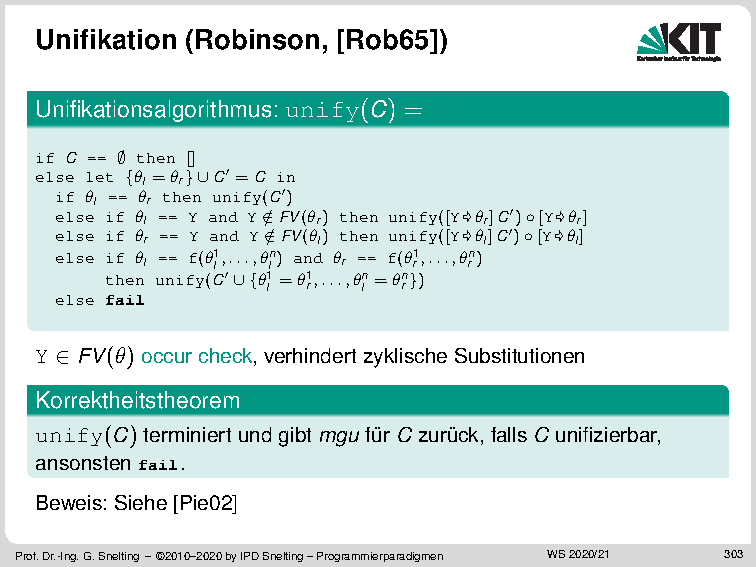
\includepdf{robinson.pdf}
}

\begin{frame}{Wiederholung: Unifikationsalgorithmus}
  \begin{equation*}
    C = \{ X = \pa{a}, Y = \functor{f}{X}, \functor{f}{Z} = Y \}
  \end{equation*}

  \only<1>{
    \begin{itemize}
      \item Problemstellung: Gleichungssystem $C$ mit baumförmigen Termen
      \begin{itemize}
        \item Bspw. Prolog-Terme, Typen
      \end{itemize}
      \item Liefert: Unifikator $\sigma_1$, der alle Gleichungen erfüllt
      \item Bspw. $\sigma_1 = \unifier{\su{X}{\pa{a}}, \su{Y}{\functor{f}{X}}, \su{Z}{X}}$
    \end{itemize}
  }

  \only<2>{
    \begin{align*}
      \texttt{unify}(C)
      &= \texttt{unify}(\{ \underline{X = \pa{a}}, Y = \functor{f}{X}, \functor{f}{Z} = Y \}) \\
      &= \texttt{unify}(\{ Y = \functor{f}{\pa{a}}, \underline{\functor{f}{Z} = Y} \}) \circ \unifier{\su{X}{\pa{a}}} \\
      &= \texttt{unify}(\{ \underline{\functor{f}{Z} = \functor{f}{\pa{a}}} \}) \circ \unifier{\su{Y}{\functor{f}{Z}}} \circ \unifier{\su{X}{\pa{a}}} \\
      &= \texttt{unify}(\{ \underline{Z = \pa{a}} \}) \circ \unifier{\su{Y}{\functor{f}{Z}}} \circ \unifier{\su{X}{\pa{a}}} \\
      &= \unifier{\su{Z}{\pa{a}}} \circ \unifier{\su{Y}{\functor{f}{Z}}} \circ \unifier{\su{X}{\pa{a}}} \\
      &= \unifier{\su{Z}{\pa{a}}, \su{Y}{\functor{f}{\pa{a}}}, \su{X}{\pa{a}}}
    \end{align*}
  }
\end{frame}

\subsection{Klausuraufgabe WS16/17 A3 a)}

\begin{frame}{Klausuraufgabe WS16/18 A3 a) (6P.)}
  \begin{align*}
    C_1 &= \{ \alpha_9 = \alpha_{10} \to \alpha_8, \alpha_9 = \alpha_4, \alpha_{10} = \texttt{bool} \} \\
    C_2 &= \{ \alpha_{12} = \alpha_{13} \to \alpha_{11}, \alpha_{12} = \alpha_4, \alpha_{13} = \texttt{int} \}
  \end{align*}

  \only<1>{
  \footnotesize
  \begin{enumerate}[i.]
    \item Geben Sie allgemeinste Unifikatoren $\sigma_1$ für $C_1$ und $\sigma_2$ für $C_2$ an.
    \item Ist auch $C_1 \cup C_2$ unifizierbar?
    \item Ist der Ausdruck\\
      \begin{equation*}\lam{a}{\lam{f}{\app{\app{f}{(\app{a}{\pa{true}})}}{(\app{a}{17})}}}\end{equation*}\\
        typisierbar? Begründen Sie ihre Antwort \emph{kurz}.
  \end{enumerate}
  }

  \only<2>{
    Geben Sie allgemeinste Unifikatoren $\sigma_1$ für $C_1$ und $\sigma_2$ für $C_2$ an.

    \begin{align*}
      \sigma_1 &= \texttt{unify}(\{ \alpha_9 = \alpha_{10} \to \alpha_8, \alpha_9 = \alpha_4, \alpha_{10} = \texttt{bool} \}) \\
               &= ... = \unifier{\su{\alpha_9}{\pa{bool} \to \alpha_8}, \su{\alpha_4}{\pa{bool} \to \alpha_8}, \su{\alpha_{10}}{\pa{bool}}} \\
      \sigma_2 &= \texttt{unify}(\{ \alpha_{12} = \alpha_{13} \to \alpha_{11}, \alpha_{12} = \alpha_4, \alpha_{13} = \texttt{int} \}) \\
               &= ... = \unifier{\su{\alpha_{12}}{\pa{int} \to \alpha_{11}}, \su{\alpha_4}{\pa{int} \to \alpha_{11}}, \su{\alpha_{13}}{\pa{int}}}
    \end{align*}
  }

  \only<3>{
    Ist auch $C_1 \cup C_2$ unifizierbar?
    \begin{align*}
      \sigma_1 &= ... = \unifier{\su{\alpha_9}{\pa{bool} \to \alpha_8}, \underline{\su{\alpha_4}{\pa{bool} \to \alpha_8}}, \su{\alpha_{10}}{\pa{bool}}} \\
      \sigma_2 &= ... = \unifier{\su{\alpha_{12}}{\pa{int} \to \alpha_{11}}, \underline{\su{\alpha_4}{\pa{int} \to \alpha_{11}}}, \su{\alpha_{13}}{\pa{int}}}
    \end{align*}

    A: Nein, da die \emph{allgemeinsten Unifikatoren} $\sigma_1$ und $\sigma_2$ einen Konflikt für $\alpha_4$ enthalten:
    $\texttt{unify}(\{ \pa{bool} = \pa{int} \}) = \texttt{fail}$
  }

  \only<4>{
    Ist der Ausdruck\\
      \begin{equation*}\lam{a}{\lam{f}{\app{\app{f}{(\app{a}{\pa{true}})}}{(\app{a}{\pa{17}})}}}\end{equation*}\\
    typisierbar? Begründen Sie ihre Antwort \emph{kurz}.

    \vfill

    A: Nein, da $a$ mit zwei verschiedenen Typen verwendet wird.
  }
\end{frame}

\begin{frame}{Typinferenz}
  Problemstellung bei Typinferenz: Zu einem gegebenen Term den passenden Typ finden.

  \begin{itemize}
    \item Struktur des Terms erkennen. Wo sind:
    \begin{itemize}
      \item Lambdas?
      \item Funktionsanwendungen?
      \item Variablen/Konstanten?
    \end{itemize}
    \item Entsprechenden Baum aufstellen.
    \item Typgleichungen finden.
    \item Gleichungssystem unifizieren.
  \end{itemize}
\end{frame}

\newcommand{\tikzmark}[3]{\tikz[baseline, remember picture]{
	\node[fill=#1,draw] (#2) {#3};
}}

\begin{frame}{Struktur von Lambda-Termen}
  Lambda-Terme bestehen aus
  \begin{itemize}
    \item \textbf<2>{Lambdas} $\lam{p}{b}$
    \item \textbf<3>{Funktionsanwendungen} $\app{x}{y}$
    \item \textbf<4>{Variablen} $x$, \textbf<5>{Konstanten} $\pa{true}, \pa{17}$
  \end{itemize}

  \only<1>{
    \begin{equation*}
      \lam{a}{\lam{f}{\app{f}{(\app{a}{\pa{true}})}}}
    \end{equation*}
  }

  \only<2>{
    \begin{equation*}
      \underbrace{
        \lam{a}{\underbrace{\lam{f}{\app{f}{(\app{a}{\pa{true}})}}}_{\text{Lambda} \atop p = f, b = \app{f}{(\app{a}{\pa{true}})}}}
      }_{
        \text{Lambda} \atop
        p = a, b = \lam{f}{\app{f}{(\app{a}{\pa{true}})}}
      }
    \end{equation*}
  }

  \only<3>{
    \begin{equation*}
      \lam{a}{\lam{f}{\underbrace{\app{f}{
        \underbrace{
         (\app{a}{\pa{true}})
        }_{\text{Anwendung} \atop x = a, y = \pa{true}}
      }}_{\text{Anwendung} \atop x = f, y = \app{a}{\pa{true}}}}}
    \end{equation*}
  }

  \only<4>{
    \begin{equation*}
      \lam{a}{\lam{f}{\app{
        \underbrace{f}_{\text{Variable}}
      }{(\app{
        \underbrace{a}_{\text{Variable}}
      }{\pa{true}})}}}
    \end{equation*}
  }

  \only<5>{
    \begin{equation*}
      \lam{a}{\lam{f}{\app{f}{(\app{a}{\underbrace{\pa{true}}_{\text{Konstante}}})}}}
    \end{equation*}
  }
\end{frame}

\begin{frame}{Lambda-Terme als Bäume}
  Wir können Lambda-Terme also als Bäume mit Lambda- und Anwendungsknoten und Variablen- und Konstantenblättern betrachten, um ihre Struktur zu untersuchen:

  \begin{columns}
    \begin{column}{0.5\textwidth}
      \begin{figure}
      \begin{tikzpicture}
        \node {$\lambda a$}
          [level distance=10mm]
          child {node {$\lambda f$}
            child {node {@}
              child {node {$f$}}
              child {node {@}
                child {node {$a$}}
                child {node {$\pa{true}$}}
              }
            }
          }
        ;
      \end{tikzpicture}
      \end{figure}
    \end{column}
    \begin{column}{0.35\textwidth}
      \begin{equation*}
        \lam{a}{\lam{f}{\app{f}{(\app{a}{\pa{true}})}}}
      \end{equation*}
    \end{column}
  \end{columns}
\end{frame}

\begin{frame}{Cheatsheet: Typisierter Lambda-Kalkül}
  \begin{mathpar}
    \inferrule{
      \Gamma{}, p : \pi \vdash b : \rho
    }{
      \Gamma \vdash \lam{p}{b} : \pi \to \rho
    } \textrm{\textsc{Abs}}
    \and
    \inferrule{
      \Gamma \vdash f : \phi \to \alpha \\
      \Gamma \vdash x : \phi
    }{
      \Gamma \vdash \app{f}{x} : \alpha
    } \textrm{\textsc{App}}
    \and
    \inferrule{
      \Gamma{}(t) = \tau
    }{
      \Gamma \vdash t : \tau
    } \textrm{\textsc{Var}}
    \and
    \inferrule{
      c \in \textsc{Const}
    }{
      \Gamma \vdash c : \tau_c
    } \textrm{\textsc{Const}}
  \end{mathpar}

  \begin{itemize}
    \item Typvariablen: $\tau$, $\alpha$, $\pi$, $\rho$
    \item Funktionstypen: $\tau_1 \to \tau_2$, rechtsassoziativ
    \item \emph{Typisierungsregeln sind eindeutig}: Eine Regel pro Termform
  \end{itemize}
\end{frame}

\begin{frame}{Was bedeuten eigentlich $\vdash$, $\Gamma$ und $:$?}
  \begin{equation*}
    \lam{a}{\lam{f}{\app{f}{(\app{a}{\pa{true}})}}}
  \end{equation*}

  Um zu einem solchen Term ein Typisierungsproblem zu beschreiben, notieren wir:

  \begin{equation*}
    \Gamma \vdash \lam{a}{\lam{f}{\app{f}{(\app{a}{\pa{true}})}}} : \tau
  \end{equation*}

  \enquote{Im \emph{Typkontext} $\Gamma$ hat der Term den Typen $\tau$.}

  \begin{itemize}
    \item $\Gamma$: Enthält Typen für freie Variablen.
    \item $... \vdash ... : ...$ --- Notation für Typisierungsproblem.
  \end{itemize}
\end{frame}

\begin{frame}{$\Gamma$ in Aktion}
  \begin{align*}
    &\Gamma \vdash a + 42 : \pa{int} \\
    &\textsc{Const} = \{ 42 \}, \tau_{42} = \texttt{int}
  \end{align*}

  Damit die Aussage \enquote{$a + 42$ hat in $\Gamma$ den Typen \texttt{int}} stimmt, müssen wir für $\Gamma$ wählen:
  
  \begin{itemize}
    \pause
    \item $\Gamma = a : \texttt{int}, + : \texttt{int} \to \texttt{int} \to \texttt{int}$
    \pause
    \item Allgemeiner: $\Gamma = a : \alpha, + : \alpha \to \texttt{int} \to \texttt{int}$
  \end{itemize}
\end{frame}

\subsection{Typisierungsregeln im Detail}

\begin{frame}{Typisierungsregel für Lambdas}
	\begin{itemize}
		\item \tikzmark{green!20}{contextL}{\enquote{Unter Einfügung des Typs $\pi$ von $p$ in den Kontext...}}
		\item \tikzmark{red!20}{bodyTypeL}{\enquote{... ist $b$ als Funktion von $p$ typisierbar.}}
	\end{itemize}

	\begin{mathpar}
		\inferrule{
			\tikzmark{green!20}{context}{$\Gamma{}, p : \pi$} \\
			\tikzmark{red!20}{bodyType}{$\vdash b : \rho$}
		}{
			\tikzmark{blue!20}{absType}{$\Gamma \vdash \lam{p}{b} : \pi \to \rho$}
                } \textrm{\textsc{Abs}}
	\end{mathpar}

	\begin{itemize}
		\item Daraus folgt:
		\item \tikzmark{blue!20}{absTypeL}{\enquote{$\lam{p}{b}$ ist eine Funktion, die $\pi$s auf $\rho$s abbildet}}
	\end{itemize}

	\tikz[overlay, remember picture]{
		\draw[->] (bodyTypeL) edge [bend left] (bodyType);
		\draw[->] (contextL) edge [bend right] (context);
		\draw[->] (absTypeL) edge [bend left] (absType);
	}
\end{frame}

\begin{frame}{Typisierungsregel für Funktionsanwendungen}
	\begin{itemize}
		\item \tikzmark{green!20}{fTypeL}{\enquote{$f$ ist im Kontext $\Gamma$ eine Funktion, die $\phi$s auf $\alpha$s abbildet.}}
		\item \tikzmark{red!20}{aTypeL}{\enquote{$x$ ist im Kontext $\Gamma$ ein Term des Typs $\phi$.}}
	\end{itemize}
	\begin{mathpar}
		\inferrule{
			\tikzmark{green!20}{fType}{$\Gamma \vdash f : \phi \to \alpha$} \\
			\tikzmark{red!20}{aType}{$\Gamma \vdash x : \phi$}
		}{
			\tikzmark{blue!20}{eType}{$\Gamma \vdash \app{f}{x} : \alpha$}
                } \textrm{\textsc{App}}
	\end{mathpar}

	\begin{itemize}
		\item Daraus folgt:
		\item \tikzmark{blue!20}{eTypeL}{\enquote{$x$ eingesetzt in $f$ ergibt einen Term des Typs $\alpha$.}}
	\end{itemize}

	\tikz[overlay, remember picture]{
		\draw[->] (fTypeL) edge [bend right] (fType);
		\draw[->] (aTypeL) edge [bend left] (aType);
		\draw[->] (eTypeL) edge [bend left] (eType);
	}
\end{frame}

\begin{frame}{Einfache Typisierungsregel für Variablen}
	\begin{itemize}
		\item \tikz[baseline, remember picture]{\node [fill=green!20,draw] (varRetL) {\enquote{Der Typkontext $\Gamma$ enthält einen Typ $\tau$ für $t$.}};}
	\end{itemize}

	\begin{mathpar}
		\inferrule{
			\tikz[baseline, remember picture]{\node[fill=green!20,draw] (varRet) {$\Gamma{}(t) = \tau$};}
		}{
			\tikz[baseline, remember picture]{\node[fill=blue!20,draw] (varShow) {
				$\Gamma \vdash t : \tau$
			};}
		} \textrm{\textsc{Var}}
	\end{mathpar}

	\begin{itemize}
		\item Daraus folgt:
		\item \tikz[baseline, remember picture]{\node [fill=blue!20,draw] (varShowL) {\enquote{Variable $t$ hat im Kontext $\Gamma$ den Typ $\tau$.}};}
	\end{itemize}

	\tikz[overlay, remember picture]{
		\draw[->] (varShowL) edge [bend left] (varShow);
		\draw[->] (varRetL) edge [bend right] (varRet);
	}
\end{frame}

% https://tex.stackexchange.com/questions/9466/color-underline-a-formula
\def\mathunderline#1#2{\color{#1}\underline{{\color{black}#2}}\color{black}}

\begin{frame}{Typisierung: Beispiel}
  \only<1>{
    \begin{mathpar}
      x : \texttt{bool} \vdash \lam{f}{\app{f}{x}} : (\texttt{bool} \to \alpha) \to \alpha
    \end{mathpar}

    \enquote{Unter der Annahme, dass $x$ den Typ \texttt{bool} hat, hat $\lam{f}{\app{f}{x}}$ den Typ $(\texttt{bool} \to \alpha) \to \alpha$.}
  }

  \only<2>{
    \begin{mathpar}
      \inferrule{
        \mathunderline{red}{x : \texttt{bool}}, \mathunderline{blue}{f} : \mathunderline{yellow}{\texttt{bool} \to \alpha} \vdash
        \mathunderline{green}{\app{f}{x}} :
        \mathunderline{orange}{\alpha}
      }{
        \mathunderline{red}{x : \texttt{bool}} \vdash \lam{\mathunderline{blue}{f}}{\mathunderline{green}{\app{f}{x}}} : (\mathunderline{yellow}{\texttt{bool} \to \alpha}) \to \mathunderline{orange}{\alpha}
      } \textsc{Abs}
    \end{mathpar}

    Pattern-Matching: Der äußerste Term ist ein Lambda, also wenden wir die $\textsc{Abs}$-Regel an.
    \begin{align*}
      \mathunderline{red}{\Gamma} &= \mathunderline{red}{x : \texttt{bool}} \\
      \mathunderline{blue}{p} &= \mathunderline{blue}{f}, \mathunderline{green}{b} = \mathunderline{green}{\app{f}{x}} \\
      \mathunderline{yellow}{\pi} &= \mathunderline{yellow}{\texttt{bool} \to \alpha} \\
      \mathunderline{orange}{\rho} &= \mathunderline{orange}{\alpha}
    \end{align*}

    \begin{mathpar}
      \inferrule{
        \mathunderline{red}{\Gamma{}}, \mathunderline{blue}{p} : \mathunderline{yellow}{\pi} \vdash \mathunderline{green}{b} : \mathunderline{orange}{\rho}
      }{
        \mathunderline{red}{\Gamma} \vdash \lam{\mathunderline{blue}{p}}{\mathunderline{green}{b}} : \mathunderline{yellow}{\pi} \to \mathunderline{orange}{\rho}
      } \textrm{\textsc{Abs}}
    \end{mathpar}
  }

  \only<3>{
    \begin{mathpar}
      \inferrule{
        \inferrule{
          \inferrule{\Gamma(f) = \texttt{bool} \to \alpha}{\Gamma \vdash f : \texttt{bool} \to \alpha} \textsc{Var} \\
          \inferrule{\Gamma(x) = \texttt{bool}           }{\Gamma \vdash x : \texttt{bool}           } \textsc{Var}
        }{
          x : \pa{bool}, f : \texttt{bool} \to \alpha \vdash \app{f}{x} : \alpha
        } \textsc{App}
      }{
        x : \texttt{bool} \vdash \lam{f}{\app{f}{x}} : (\texttt{bool} \to \alpha) \to \alpha
      } \textsc{Abs}
    \end{mathpar}

    \begin{equation*}
      \Gamma = x : \pa{bool}, f : \texttt{bool} \to \alpha
    \end{equation*}

    \begin{columns}
      \begin{column}{0.5\textwidth}
        \begin{figure}
          \begin{tikzpicture}
            \node {$\lambda f$}
              [level distance=10mm]
              child {node {@}
                child {node {f}}
                child {node {x}}
              }
            ;
          \end{tikzpicture}
        \end{figure}
      \end{column}
      \begin{column}{0.35\textwidth}
        \begin{equation*}
          \lam{f}{\app{f}{x}}
        \end{equation*}
      \end{column}
    \end{columns}
  }
\end{frame}

\subsection{Von Typisierungsregeln zu Typinferenz}

\begin{frame}{Von Typisierungsregeln zu Typinferenz}
  Beim inferieren wird das Pattern-matching der Typen durch die \emph{Unifikation} übernommen.
  Deswegen schreiben wir anstelle von konkreten Typen immer $\alpha_i$ und merken uns die Gleichungen für später:

  \only<1>{
    \begin{equation*}
      \inferrule{
        \Gamma{}, p : \pi \vdash b : \rho
      }{
        \Gamma \vdash \lam{p}{b} : \pi \to \rho
      } \textrm{\textsc{Abs}}
      \;\;
      \leadsto
      \;\;
      {\inferrule{
        \Gamma{}, p : \alpha_j \vdash b : \alpha_k
      }{
        \Gamma \vdash \lam{p}{b} : \alpha_i
      } \textrm{\textsc{Abs}} \atop
      \{ \alpha_i = \alpha_j \to \alpha_k \}}
    \end{equation*}
  }

  \only<2>{
    \begin{equation*}
      \inferrule{
        \Gamma \vdash f : \phi \to \alpha \\
        \Gamma \vdash x : \phi
      }{
        \Gamma \vdash \app{f}{x} : \alpha
      } \textrm{\textsc{App}}
      \;\;
      \leadsto
      \;\;
      {\inferrule{
        \Gamma \vdash f : \alpha_j \\
        \Gamma \vdash x : \alpha_k
      }{
        \Gamma \vdash \app{f}{x} : \alpha_i
      } \textrm{\textsc{App}} \atop
      \{ \alpha_j = \alpha_k \to \alpha_i \}}
    \end{equation*}
  }

  \only<3>{
    \begin{equation*}
      \inferrule{
        \Gamma{}(t) = \tau
      }{
        \Gamma \vdash t : \tau
      } \textrm{\textsc{Var}}
      \;\;
      \leadsto
      \;\;
      {\inferrule{
        \Gamma{}(t) = \alpha_j
      }{
        \Gamma \vdash t : \alpha_i
      } \textrm{\textsc{Var}} \atop
      \{ \alpha_i = \alpha_j \}}
    \end{equation*}
  }
\end{frame}

\subsection{Hindley-Milner-Algorithmus}

\begin{frame}{Algorithmus zur Typinferenz}
	\begin{itemize}
		\item Stelle Typherleitungsbaum auf
		\begin{itemize}
			\item In jedem Schritt werden neue Typvariablen $\alpha_i$ angelegt
			\item Statt die Typen direkt im Baum einzutragen, werden Gleichungen in einem Constraint-System eingetragen
		\end{itemize}
		\item Unifiziere Constraint-System zu einem Unifikator
		\begin{itemize}
			\item Robinson-Algorithmus, im Grunde wie bei Prolog
                        \item I.d.R.: Allgemeinster Unifikator (mgu)
		\end{itemize}
	\end{itemize}

	\begin{columns}
		\scriptsize
		\begin{column}{0.3\textwidth}
                  \begin{mathpar}
    \inferrule{
      \Gamma{}(t) = \alpha_j
    }{
      \Gamma \vdash t : \alpha_i
    } \textrm{\textsc{Var}}
                  \end{mathpar}

                  \center
                        Constraint:\\$\{ \alpha_i = \alpha_j \}$
		\end{column}
		\begin{column}{0.3\textwidth}
                  \begin{mathpar}
    \inferrule{
      \Gamma \vdash f : \alpha_j \\
      \Gamma \vdash x : \alpha_k
    }{
      \Gamma \vdash \app{f}{x} : \alpha_i
    } \textrm{\textsc{App}}
                  \end{mathpar}
\center
			Constraint:\\$\{ \alpha_j = \alpha_k \to \alpha_i \}$
		\end{column}
		\begin{column}{0.3\textwidth}
                  \begin{mathpar}
    \inferrule{
      \Gamma{}, p : \alpha_j \vdash b : \alpha_k
    }{
      \Gamma \vdash \lam{p}{b} : \alpha_i
    } \textrm{\textsc{Abs}}
                  \end{mathpar}
                        \center
			Constraint:\\$\{ \alpha_i = \alpha_j \to \alpha_k \}$
		\end{column}
	\end{columns}
\end{frame}

\begin{frame}{Herleitungsbaum: Beispiel}
  \only<1>{
    \begin{mathpar}
      \vdash \lam{x}{\lam{y}{x}} : \alpha_1
    \end{mathpar}

    Beispielhafte Aufgabenstellung: Finde den Typen $\alpha_1$.
  }

  \only<2>{
    \begin{mathpar}
      \inferrule{
        \mathunderline{red}{x} : \alpha_2 \vdash \mathunderline{blue}{\lam{y}{x}} : \alpha_3
      }{
        \vdash \lam{\mathunderline{red}{x}}{\mathunderline{blue}{\lam{y}{x}}} : \alpha_1
      } \textsc{Abs}
    \end{mathpar}

    Typgleichungen:

    \begin{equation*}
      C = \{ \underline{\alpha_1 = \alpha_2 \to \alpha_3} \}
    \end{equation*}
  }

  \only<3>{
    \begin{mathpar}
      \inferrule{
        \inferrule{
          \mathunderline{red}{x : \alpha_2}, \mathunderline{blue}{y} : \alpha_4 \vdash \mathunderline{orange}{x} : \alpha_5
        }{
          \mathunderline{red}{x : \alpha_2} \vdash \lam{\mathunderline{blue}{y}}{\mathunderline{orange}{x}} : \alpha_3
        } \textsc{Abs}
      }{
        \vdash \lam{x}{\lam{y}{x}} : \alpha_1
      } \textsc{Abs}
    \end{mathpar}

    Typgleichungen:

    \begin{align*}
      C = \{ & \alpha_1 = \alpha_2 \to \alpha_3 \\
           , & \underline{\alpha_3 = \alpha_4 \to \alpha_5} \}
    \end{align*}
  }

  \only<4>{
    \begin{mathpar}
      \inferrule{
        \inferrule{
          \inferrule{
            (\mathunderline{red}{x : \alpha_2, y : \alpha_4})(\mathunderline{blue}{x}) = \alpha_2
          }{
            \mathunderline{red}{x : \alpha_2, y : \alpha_4} \vdash \mathunderline{blue}{x} : \alpha_5
          } \textsc{Var}
        }{
          x : \alpha_2 \vdash \lam{y}{x} : \alpha_3
        } \textsc{Abs}
      }{
        \vdash \lam{x}{\lam{y}{x}} : \alpha_1
      } \textsc{Abs}
    \end{mathpar}

    Typgleichungen:
    
    \begin{align*}
      C = \{ & \alpha_1 = \alpha_2 \to \alpha_3 \\
           , & \alpha_3 = \alpha_4 \to \alpha_5 \\
           , & \underline{\alpha_5 = \alpha_2} \}
    \end{align*}
  }
\end{frame}

\begin{frame}{Herleitungsbaum: Aufgabe}
  \begin{mathpar}
    \inferrule{
      ...
    }{
      \vdash \lam{f}{\app{f}{(\lam{x}{x})}} : \alpha_1
    } \textsc{Abs}
  \end{mathpar}

  Findet den Typen $\alpha_1$. Teilpunkte gibt es für:

  \begin{itemize}
    \item Herleitungsbaum,
    \item Typgleichungsmenge $C$,
    \item Unifikation per Robinsonalgorithmus.
  \end{itemize}
\end{frame}

\begin{frame}{Herleitungsbaum: Aufgabe}
\begin{mathpar}
\inferrule{
\inferrule{
\inferrule{
(f : \alpha_2)(f) = \alpha_2
}{
f : \alpha_2 \vdash f : \alpha_4
} \textsc{Var}
\\
\inferrule{
\inferrule{
\Gamma(x) = \alpha_6
}{
\Gamma \vdash x : \alpha_7
} \textsc{Var}
}{
f : \alpha_2 \vdash \lam{x}{x} : \alpha_5
} \textsc{Abs}
}{
f : \alpha_2 \vdash \app{f}{(\lam{x}{x})} : \alpha_3
} \textsc{App}
}{
\vdash \lam{f}{\app{f}{(\lam{x}{x})}} : \alpha_1
} \textsc{Abs}\\
\Gamma = f : \alpha_2, x : \alpha_6
\end{mathpar}

\begin{align*}
  C = \{ & \alpha_1 = \alpha_2 \to \alpha_3, \alpha_4 = \alpha_5 \to \alpha_3, \\
           & \alpha_2 = \alpha_4, \\
           & \alpha_5 = \alpha_6 \to \alpha_7, \alpha_6 = \alpha_7 \}
\end{align*}
\end{frame}

\section{\textsc{Let}-Polymorphismus}

\begin{frame}{\textsc{Let}-Polymorphismus: Motivation}
  \begin{equation*}
    \lam{f}{\app{f}{f}}
  \end{equation*}

  \begin{itemize}
    \item Diese Funktion verwendet $f$ auf zwei Arten:
    \begin{itemize}
      \item $\alpha \to \alpha$: Rechte Seite.
      \item $(\alpha \to \alpha) \to (\alpha \to \alpha)$: Linke Seite, nimmt $f$ als Argument und gibt es zurück.
    \end{itemize}
    \pause
    \item Problem: $\alpha \to \alpha$ und $(\alpha \to \alpha) \to (\alpha \to \alpha)$ sind nicht unifizierbar!
    \begin{itemize}
      \item \enquote{occurs check}: $\alpha$ darf sich nicht selbst einsetzen.
    \end{itemize}
  \item Idee: Bei jeder Verwendung eines polymorphen Typen erzeugen wir \emph{neue Typvariablen}, um diese Beschränkung zu umgehen.
  \end{itemize}
\end{frame}

\begin{frame}{Typschemata und Instanziierung}
  \only<1>{
    \begin{itemize}
      \item Idee: Bei jeder Verwendung eines polymorphen Typen erzeugen wir \emph{neue Typvariablen}, um diese Beschränkung zu umgehen.
      \item Ein \emph{Typschema} ist ein Typ, in dem manche Typvariablen allquantifiziert sind:
    \end{itemize}

    \begin{align*}
      \phi     & = \forall \alpha_1 . \; ... \; \forall \alpha_n . \tau \\
      \alpha_i & \in FV(\tau)
    \end{align*}

    \begin{itemize}
      \item \emph{Typschemata kommen bei uns immer nur in Kontexten vor!}
      \item Beispiele:
      \begin{itemize}
        \item $\forall \alpha . \alpha \to \alpha$
        \item $\forall \alpha . \alpha \to \beta \to \alpha$
      \end{itemize}
    \end{itemize}

  }

  \only<2>{
    \begin{itemize}
      \item Ein Typschema spannt eine Menge von Typen auf, mit denen es \emph{instanziiert} werden kann:
    \end{itemize}

    \begin{align*}
      \forall \alpha . \alpha \to \alpha & \succeq \text{int} \to \text{int} \\
      \forall \alpha . \alpha \to \alpha & \succeq \tau \to \tau \\
      \forall \alpha . \alpha \to \alpha & \not\succeq \tau \to \sigma \\
      \forall \alpha . \alpha \to \alpha & \not\succeq \tau \to \tau \to \tau \\
      \forall \alpha . \alpha \to \alpha & \succeq (\tau \to \tau) \to (\tau \to \tau)
    \end{align*}
  }
\end{frame}

\begin{frame}{\textsc{Let}-Polymorphismus}
  \only<1>{
    Um Typschemata bei der Inferenz zu verwenden, müssen wir zunächst die Regel für Variablen anpassen:

    \begin{mathpar}
      \inferrule{
        \Gamma(x) = \phi \\
        \phi \succeq_{\text{frische $\alpha_i$}} \tau
      }{
        \Gamma \vdash x : \alpha_j
      } \textsc{Var} \\
      \text{Constraint:} \; \{ \alpha_j = \tau \}
    \end{mathpar}

    \begin{itemize}
      \item $\succeq_\text{frische $\alpha_i$}$ instanziiert ein Typschema mit $\alpha_i$, die noch nicht im Baum vorkommen.
      \item Jetzt brauchen wir noch eine Möglichkeit, Typschemata zu erzeugen.
    \end{itemize}
  }

  \only<2>{
    Mit einen \textsc{Let}-Term wird ein Typschema eingeführt:

    \begin{mathpar}
      \inferrule{
        \Gamma \vdash t_1 : \alpha_i \\
        \Gamma' \vdash t_2 : \alpha_j
      }{ 
        \Gamma \vdash \texttt{let} \;\; x = t_1 \;\; \texttt{in} \;\; t_2 : \alpha_k
      } \textsc{Let}
    \end{mathpar}

    \pause

    \begin{align*}
      \sigma_{let} &= mgu(C_{let}) \\
           \Gamma' &= \sigma_{let}(\Gamma), x : ta(\sigma_{let}(\alpha_i), \sigma_{let}(\Gamma)) \\
          C'_{let} &= \{ \alpha_n = \sigma_{let}(\alpha_n) \mid \sigma_{let}(\alpha_n) \;\; \text{ist definiert} \}
    \end{align*}

    Constraints: $C'_{let} \cup C_{body} \cup \{ a_j = a_k \}$
  }
\end{frame}

\begin{frame}{Beispiel: \textsc{Let}-Polymorphismus}
    \scriptsize
    \begin{mathpar}
      \inferrule{
        \inferrule{
          ...
        }{
          \vdash \lam{x}{x} : \alpha_2
        } \textsc{Abs} \\
        \inferrule{
          \inferrule{
            \Gamma'(f) = \forall \alpha_5 . \alpha_5 \to \alpha_5 \\\\
            \succeq \alpha_8 \to \alpha_8
          }{
            \Gamma' \vdash f : \alpha_6
          } \textsc{Var} \\
          \inferrule{
            \Gamma'(f) = \forall \alpha_5 . \alpha_5 \to \alpha_5 \\\\
            \succeq \alpha_9 \to \alpha_9
          }{
            \Gamma' \vdash f : \alpha_7
          } \textsc{Var}
        }{
          \Gamma' \vdash \app{f}{f} : \alpha_3
        } \textsc{App}
      }{ 
        \vdash \texttt{let} \;\; f = \lam{x}{x} \;\; \texttt{in} \;\; \app{f}{f} : \alpha_1
      } \textsc{Let}
    \end{mathpar}

    \begin{align*}
           C_{let} &= \{ \alpha_2 = \alpha_4 \to \alpha_5, \alpha_4 \to \alpha_5 \} \\
      \sigma_{let} &= \unifier{\su{\alpha_2}{\alpha_5 \to \alpha_5}, \su{\alpha_4}{\alpha_5}} \\
      \Gamma'      &= x : \forall \alpha_5 . \alpha_5 \to \alpha_5 \\
          C'_{let} &= \{ \alpha_2 = \alpha_5 \to \alpha_5, \alpha_4 = \alpha_5 \} \\
          C_{body} &= \{ \alpha_6 = \alpha_7 \to \alpha_3, \alpha_6 = \alpha_8 \to \alpha_8, \alpha_7 = \alpha_9 \to \alpha_9 \} \\
                 C &= C'_{let} \cup C_{body} \cup \{ \alpha_3 = \alpha_1 \}
    \end{align*}
\end{frame}

\section{Einführung in Compilerbau}

% Aufgaben:
% Nicht-SLL(1)-Teilmenge von JSON-Subset ist SLL(n) für n \in 1, 2?
% Rekursiver Abstieg für JSON-Subset
% Rekursiver Abstieg für Klausuraufgabenliste
% Java Bytecode

\begin{frame}{Compiler in ProPa}
	\begin{itemize}
		\item Ein bisschen...
		\begin{itemize}
			\item Lexikalische Analyse (Tokenisierung)
			\item Syntaktische Analyse (Parsen)
			\item \textcolor{gray}{Semantische Analyse (Optimierung)}
			\item Codegenerierung
		\end{itemize}
		\pause
		\item Klausur:
		\begin{itemize}
			\item SLL(k)-Form beweisen
			\item Rekursiven Abstiegsparser schreiben/vervollständigen
			\item First/Follow-Mengen berechnen
			\item Java-Bytecode
				% Zeigen: Java-BC-Aufgabe (16SS), Code-Generierung nächste Mittwoch und Freitag (findet noch statt)
		\end{itemize}
	\end{itemize}
\end{frame}

\subsection{Syntaktische Analyse (18WS)}

\begin{frame}{Syntaktische Analyse (18WS)}
	\begin{align*}
		SGML \to & \;\; \textrm{\texttt{< id >}} \;\; Children \;\; \textrm{\texttt{< / >}}\\
		Children \to & \;\; \epsilon \mid SGML \;\; Children
	\end{align*}

	\begin{equation*}
		\{\textrm{\texttt{<id><id></><id></></>}},\;\;\textrm{\texttt{<id></>}},\;\;...\} \in G
	\end{equation*}

	\pause
	\begin{itemize}
		\item Begründen Sie formal, dass die obige Grammatik nicht in $\textrm{SLL}(1)$-Form ist (3P.).
		\pause
		\item Entwickeln Sie für [eine linksfaktorisierte Version der obigen Grammatik] einen rekursiven Abstiegsparser (16P.).
	\end{itemize}
\end{frame}

\begin{frame}{Java-Bytecode (16SS)}
	\footnotesize
	Übersetzen Sie folgenden Java-Programmausschnitt in Java-Bytecode (10P.):

	\code{code/bytecode16ss.java}

	\pause
	Hinweise:

	\begin{itemize}
		\item Codeerzeugung für bedingte Sprünge: Folien 447ff.
		\item Um eine Bedingung der Form \texttt{!cond} zu übersetzen, reicht es, \texttt{cond} zu übersetzen und die Sprungziele anzupassen.
	\end{itemize}
\end{frame}

% Aufgaben:
% Nicht-SLL(1)-Teilmenge von JSON-Subset ist SLL(n) für n \in 1, 2?
% Rekursiver Abstieg für JSON-Subset
% Rekursiver Abstieg für Klausuraufgabenliste
% Java Bytecode

\section{Compiler}

\subsection{Motivation}

\begin{frame}{Compiler: Motivation}
	\begin{itemize}
		\item Maschine(-nmodell) versteht i.d.R. eingeschränkten Instruktionssatz
		\begin{itemize}
			\item Es gibt/gab zwar auch mal CISC-Maschinen, heute ist sind aber RISC(-ähnliche) Prozessoren am weitesten verbreitet
			\item Gründe: RISC-Prozessoren sind wesentlich einfacher (= billiger) zu bauen
		\end{itemize}
		\item Programme in Maschinensprache sind i.d.R. für Menschen nicht einfach zu Schreiben.
		\pause
		\item Also: Erfinde einfacher zu Schreibende ($\approx$ mächtigere) Sprache, die dann in die Sprache der Maschine übersetzt wird.
		\item Diesen Übersetzungsschritt sollte optimalerweise ein Programm erledigen, da wir sonst auch einfach direkt Maschinensprache-Programme schreiben können.
	\end{itemize}
\end{frame}

\begin{frame}{Compiler}
	\begin{itemize}
		\item Übersetzer für formale Sprachen nennt man \emph{Compiler}
		\item Beispiele:
		\begin{itemize}
			\item C, Haskell, Rust, Go $\to$ X86
			\item Java, Clojure, Kotlin $\to$ Java-Bytecode
			\item TypeScript $\to$ JavaScript
			\item \textcolor{gray}{Python $\to$ Python-AST}
		\end{itemize}
		\pause
		\item \textcolor{gray}{Interpreter kann man auch als Compiler kategorisieren, sie zählen aber i.A. nicht dazu}
		\pause
		\item Single-pass vs. Multi-pass
		\begin{itemize}
			\item Single-pass: Eingabe wird einmal gelesen, Ausgabe währenddessen erzeugt (ältere Compiler)
			\item Multi-pass: Eingabe wird in Zwischenschritten in verschiedene Repräsentationen umgewandelt
			\begin{itemize}
				\item Quellsprache, Tokens, AST, Zwischensprache, Zielsprache
			\end{itemize}
		\end{itemize}
	\end{itemize}
\end{frame}

\subsection{Lexikalische Analyse}

\begin{frame}{Lexikalische Analyse}
	\begin{columns}
		\begin{column}{0.5\textwidth}
			\code{code/lexinput.java}
		\end{column}
		\begin{column}{0.5\textwidth}
			\code{code/lexoutput.java}
		\end{column}
	\end{columns}

	\begin{itemize}
		\item Lexikalische Analyse (Tokenisierung) verarbeitet eine Zeichensequenz in eine Liste von \emph{Tokens}.
		\item Tokens sind Zeichengruppen, denen eine Semantik innewohnt:
		\begin{itemize}
			\item \texttt{int} --- Typ einer Ganzzahl
			\item \texttt{=} --- Zuweisungsoperator
			\item \texttt{x1} --- Variablen- oder Methodenname
			\item \texttt{123} --- Literal einer Ganzzahl
			\item \texttt{"123"} --- String-Literal
			\item etc.
		\end{itemize}
		\item Lösbar mit regulären Ausdrücken, Automaten
	\end{itemize}
\end{frame}

\subsection{Syntaktische Analyse}

\begin{frame}{Syntaktische Analyse}
	\begin{itemize}
		\item Syntaktische Analyse stellt die unterliegende Struktur der bisher linear gelesenen Eingabe fest:
		\begin{itemize}
			\item Blockstruktur von Programmen
			\item Baumstruktur von HTML-Dateien
			\item Header, Inhalt-Struktur von Mails
			\item Verschachtelte mathematische Ausdrücke
		\end{itemize}
		\item Syntaktische Analyse ist das größte Compiler-Thema in PP.
		\pause
		\item Übliche Vorgehensweise (in PP):
		\begin{itemize}
			\item Grammatik $G$ erfinden
			\item ggf. $G$ in einfache Form $G'$ bringen
			\item rekursiven Abstiegsparser für $G'$ implementieren
		\end{itemize}
		\item Alternativ: Parser-Kombinatoren, Yacc, etc.
	\end{itemize}
\end{frame}

\begin{frame}{Beispiel: Mathematische Ausdrücke}
	\begin{columns}
		\begin{column}{0.3\textwidth}
			\begin{equation*}
				1 + 5 * 7 + 6
			\end{equation*}
		\end{column}
		\begin{column}{0.8\textwidth}
                  \Tree [.E [.E 1 ] + [.E [.E [ [.E 5 ] * [.E 7 ] ] + [.E 6 ] ] ] ]
		\end{column}
	\end{columns}

	\begin{itemize}
		\item Zu beachten: Punkt-vor-Strich (Präzedenz), Klammerung, etc.
		\item Nicht mehr mit regulären Ausdrücken lösbar
		\item \enquote{Offensichtliche} Grammatik oft nicht einfach zu Parsen
	\end{itemize}
\end{frame}

\begin{frame}{Beispiel: Mathematische Ausdrücke}
	\begin{equation*}
		E \to \;\; \textrm{\texttt{num}} \mid \textrm{\texttt{(}} \;\; E \;\; \textrm{\texttt{)}}
		 \mid E \;\; \textrm{\texttt{+}} \;\; E
		 \mid E \;\; \textrm{\texttt{*}} \;\; E
	\end{equation*}

	\pause

	\begin{columns}
		\begin{column}{0.5\textwidth}
			\begin{figure}
				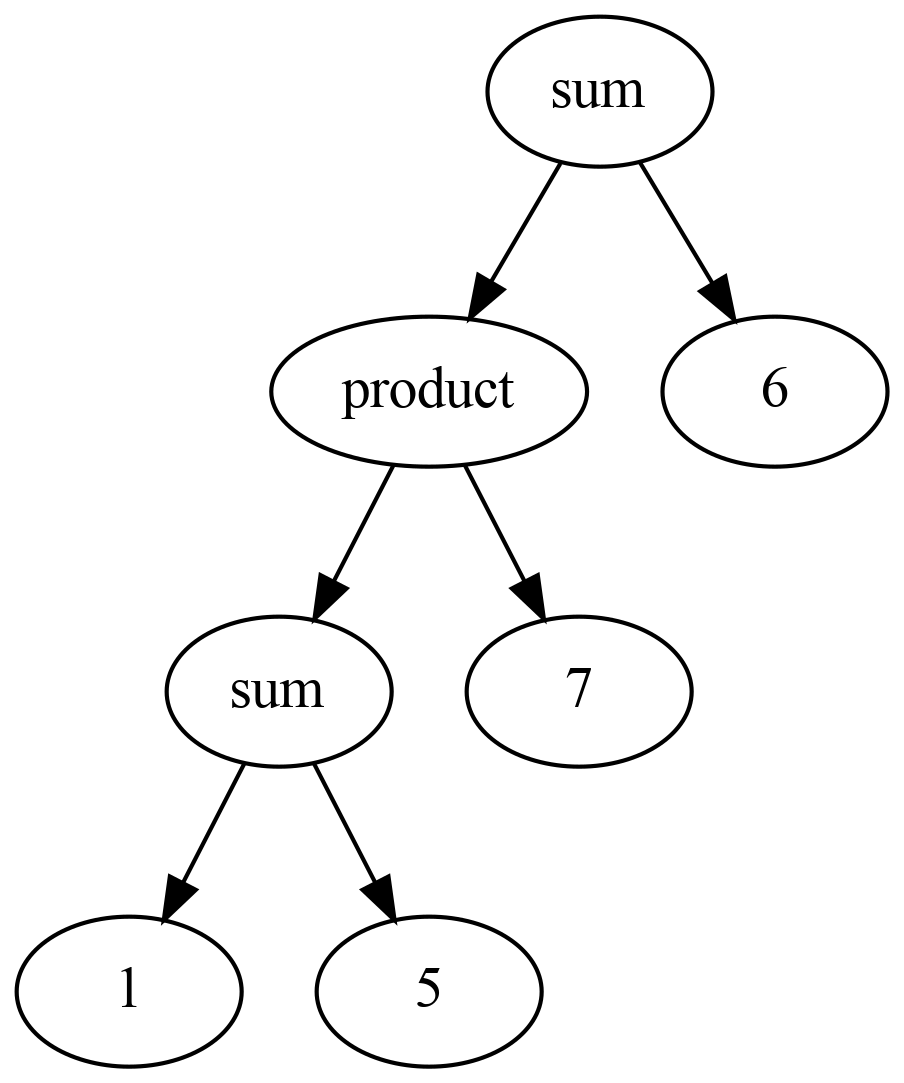
\includegraphics[width=0.65\textwidth]{images/baumstruktur2.png}
			\end{figure}
		\end{column}
		\begin{column}{0.5\textwidth}
			\begin{figure}
				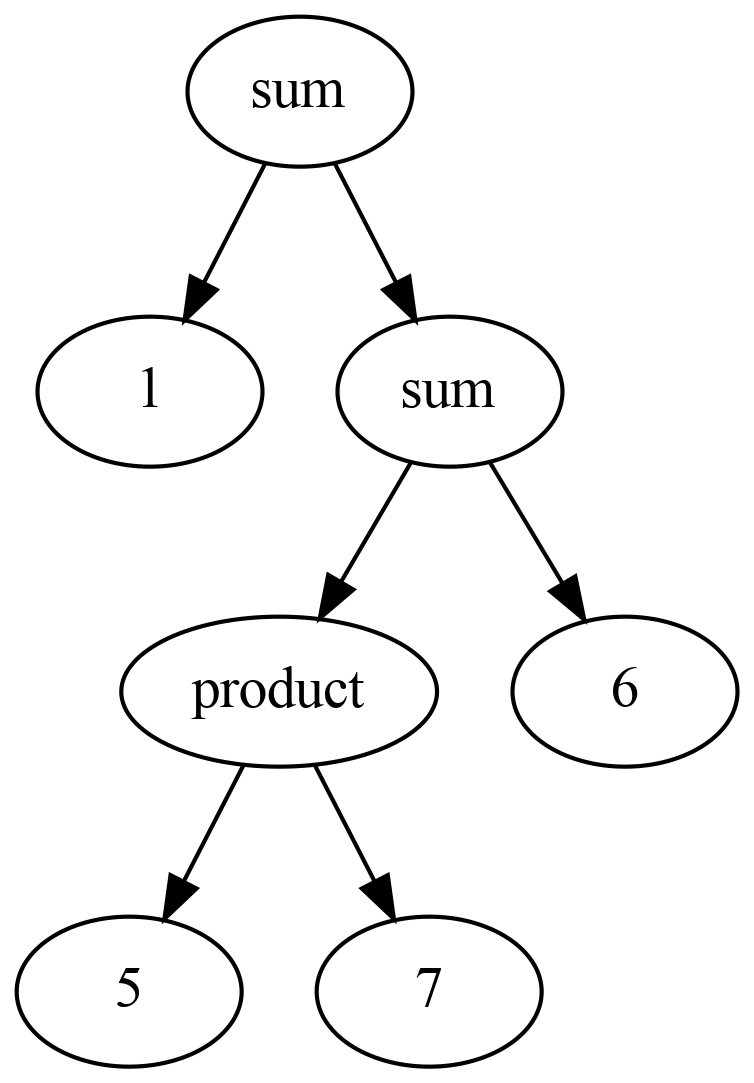
\includegraphics[width=0.65\textwidth]{images/baumstruktur.png}
			\end{figure}
		\end{column}
	\end{columns}

	\pause

	\begin{itemize}
		\item Ableitungsbaum nicht eindeutig $\leadsto$ schlecht
		\item Ableitungsbaum garantiert nicht Punkt-vor-Strich $\leadsto$ schlecht
	\end{itemize}
\end{frame}

\begin{frame}{Präzedenz, Linksfaktorisierung}
	Wie zeichnen sich \enquote{gute} Grammatiken aus?
	\pause

	Operatorpräzedenz schon in Grammatik definiert:
	\begin{align*}
		E \to & \;\; E \;\; \textrm{\texttt{+}} \;\; T \mid E \;\; \textrm{\texttt{-}} \;\; T \mid T\\
		T \to & \;\; T \;\; \textrm{\texttt{*}} \;\; F \mid T \;\; \textrm{\texttt{/}} \;\; F \mid F\\
		F \to & \;\; \textrm{\texttt{num}} \; | \; \textrm{\texttt{(}} \;\; E \;\; \textrm{\texttt{)}}
	\end{align*}

	\pause

	Vermeidung von Linksrekursion (Linksfaktorisierung):
	\begin{align*}
		E     \to & \;\; T \;\; EList\\
		EList \to & \;\; \epsilon \mid \textrm{\texttt{+}} \;\; T \;\; EList \mid \textrm{\texttt{-}} \;\; T \;\; EList\\
		T     \to & \;\; F \;\; TList\\
		TList \to & \;\; \epsilon \mid \textrm{\texttt{*}} \;\; F \;\; TList \mid \textrm{\texttt{/}} \;\; F \;\; TList\\
		F \to & \;\; \textrm{\texttt{num}} \; | \; \textrm{\texttt{(}} \;\; E \;\; \textrm{\texttt{)}}
	\end{align*}
\end{frame}

\begin{frame}{First-/Followmenge, Indizmenge}
	\footnotesize

	\begin{align*}
		EList \to & \;\; \epsilon \mid \textrm{\texttt{+}} \;\; T \;\; EList \mid \textrm{\texttt{-}} \;\; T \;\; EList
	\end{align*}
	
	Wie können wir bspw. bei $EList$ entscheiden, welche Produktion anzuwenden ist?
	\pause
	\begin{itemize}
		\item $\leadsto$ definiere \emph{Indizmenge} $IM_k(A \to \alpha) = \textrm{First}_k(\alpha \textrm{Follow}_k(A))$
		\item Wenn nächste $k$ Token in $IM_k(EList \to \phi)$ $\leadsto$ weiter mit $\phi$
		\pause
		\item $IM_1(EList \to \; \epsilon) = \textrm{First}_1(\epsilon \textrm{Follow}_1(EList)) = \{ \textrm{\texttt{)}}, \textrm{\texttt{\#}} \}$
		\item $IM_1(EList \to \; \textrm{\texttt{+}} \;\; T \;\; EList) = \textrm{First}_1(\textrm{\texttt{+}} \; T \; EList \; \textrm{Follow}_1(EList)) = \{ \textrm{\texttt{+}} \}$
		\item $IM_1(EList \to \; \textrm{\texttt{-}} \;\; T \;\; EList) = \textrm{First}_1(\textrm{\texttt{-}} \; T \; EList \; \textrm{Follow}_1(EList)) = \{ \textrm{\texttt{-}} \}$
		\pause
		\item $\textrm{First}_k(A)$: Menge an möglichen ersten $k$ Token in $A$
		\item $\textrm{Follow}_k(A)$: Menge an möglichen ersten $k$ Token nach $A$
	\end{itemize}
\end{frame}

\begin{frame}{SLL-Kriterium}
	Grammatik ist in $\textrm{SLL}(k)$-Form\\
	$:\Leftrightarrow \forall A \to \alpha, A \to \beta \in P: IM_k(A \to \alpha) \cap IM_k(A \to \beta) = \emptyset$

	\begin{itemize}
		\item $\textrm{SLL}(k)$: Bei jedem Nichtterminal muss die zu wählende Produktion an den nächsten $k$ Token wählbar sein.
		\item Nichtterminale mit nur einer Produktion sind hier irrelevant
		\item Schwierig daran: $\textrm{Follow}$-Mengen berechnen
	\end{itemize}
	\pause
	\begin{align*}
		E \to & \;\; E \;\; \textrm{\texttt{+}} \;\; T \mid E \;\; \textrm{\texttt{-}} \;\; T \mid T\\
		T \to & \;\; T \;\; \textrm{\texttt{*}} \;\; F \mid T \;\; \textrm{\texttt{/}} \;\; F \mid F\\
		F \to & \;\; \textrm{\texttt{num}} \; | \; \textrm{\texttt{(}} \;\; E \;\; \textrm{\texttt{)}}
	\end{align*}
	
	\begin{itemize}
		\item Begründet formal, dass obige Grammatik nicht $\textrm{SLL}(1)$.
		\item Berechnet $\textrm{Follow}_1(N)$ für $N \in \{ E, T, F \}$.
	\end{itemize}
\end{frame}

\begin{frame}{Rekursive Abstiegsparser}
	\footnotesize
	\begin{align*}
		E     \to & \;\; T \;\; EList\\
		EList \to & \;\; \epsilon \mid \textrm{\texttt{+}} \;\; T \;\; EList \mid \textrm{\texttt{-}} \;\; T \;\; EList\\
		T     \to & \;\; F \;\; TList\\
		TList \to & \;\; \epsilon \mid \textrm{\texttt{*}} \;\; F \;\; TList \mid \textrm{\texttt{/}} \;\; F \;\; TList\\
		F \to & \;\; \textrm{\texttt{num}} \; | \; \textrm{\texttt{(}} \;\; E \;\; \textrm{\texttt{)}}
	\end{align*}
	\begin{itemize}
		\item Yay, unsere Grammatik hat jetzt $\textrm{SLL}(1)$-Form!
		\item Aber was bringt das?
		\pause
		\item $G$ ist jetzt einfach ausprogrammierbar:
		\begin{itemize}
			\item 1 Methode per Nichtterminal: \texttt{parseE()}, \texttt{parseEList()}, ...
			\item \texttt{Token[k]}-Instanzattribut für $k$ langen Lookahead
			\item \texttt{expect(TokenType)}-Methode, um Token zu verarbeiten
		\end{itemize}
		\pause
		\item Vervollständigt \texttt{demos/java/exprparser/ExprParser.java}!
	\end{itemize}
\end{frame}

\subsection{Semantische Analyse}

\begin{frame}{Semantische Analyse}
	\begin{itemize}
		\item PP beschäftigt sich (bis auf Typinferenz) nur kurz mit semantischer Analyse
		\item Hier geht es um Optimierungen, Typchecks, etc.
		\item $\leadsto$ weiterführende (Master-)Vorlesungen am IPD
	\end{itemize}
\end{frame}

\section{Ende}

\begin{frame}{Ende}
  \begin{itemize}
    \item Di, 16.02.: Letztes Tut
    \item Mi, 17.02.: Letzte Vorlesung
    \item Themen: Mehr Syntaxanalyse (Beispiele), Codeerzeugung
  \end{itemize}
\end{frame}

\end{document}
